% Muscle activation control content in this repository's Gemini-portrait format.
\documentclass[final]{beamer}
\usepackage[T1]{fontenc}
\usepackage{lmodern}
\usepackage[size=custom,width=91,height=122,scale=0.90]{beamerposter}
\usetheme{gemini}
\usecolortheme{heriotwatt}
\usepackage{graphicx}
\usepackage{booktabs}
\usepackage{tikz}
\usepackage{amsmath}
\graphicspath{{figures/}}

% Original repository geometry: left column, wide upper-right panel,
% then two columns beneath that panel.
\newlength{\sepwidth}
\newlength{\colwidth}
\newlength{\doublecolwidth}
\setlength{\sepwidth}{0.025\paperwidth}
\setlength{\colwidth}{0.3\paperwidth}
\setlength{\doublecolwidth}{0.625\paperwidth}
\newcommand{\separatorcolumn}{\begin{column}{\sepwidth}\end{column}}
\newcommand{\dg}{$^\circ$}
\newcommand{\hi}[1]{\textcolor{darkblue}{\textbf{#1}}}
\title{Non-Smooth Equilibria in Hill-Type Muscle Models:\\
a Quantified Consequence for Linearization-Based Control}
\author{Alan Royce Gabriel Samuel}
\institute{Indian Institute of Technology Madras, Chennai, India\\
\texttt{bs22b001@smail.iitm.ac.in}}

\begin{document}
\begin{frame}[t]
\begin{columns}[t]
\separatorcolumn
\begin{column}{\colwidth}
\begin{alertblock}{The problem}
Linearization-based controllers assume a well-defined local model at an
operating point. In the Hill-type formulation studied here, equilibria lie
on both activation and force--velocity switches.

\textbf{One equilibrium therefore has four directional linear models.}
Does choosing the wrong branch matter for prediction and feedback control?
\end{alertblock}

\begin{block}{Musculoskeletal model}
A single elbow joint drives a forearm--hand pendulum against gravity.
The actuator is a rigid-tendon Hill-type brachialis model, with Thelen
activation dynamics, Holzbaur muscle parameters and a moment arm digitized
from Murray et al.

The reference equilibrium is \textbf{60\dg\ and activation 0.113}.
All four local branches are stable; the issue is their differing slopes.
\begin{figure}
\centering
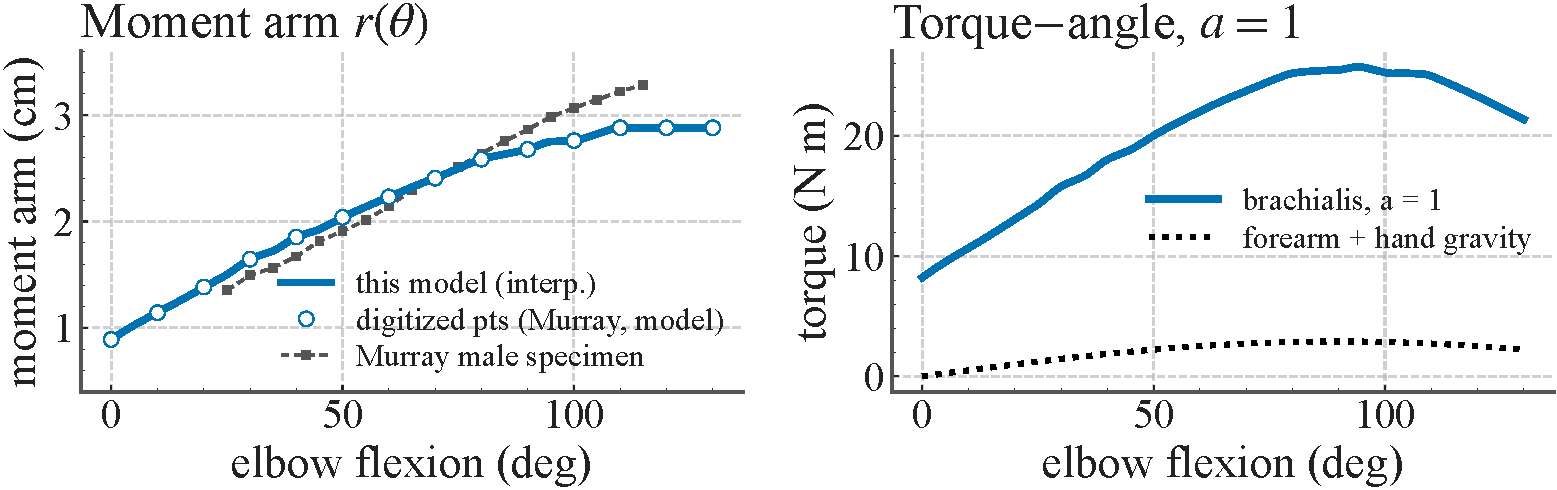
\includegraphics[width=\linewidth]{fig6_validation.pdf}
\caption{Moment-arm and torque--angle checks. Brachialis peaks at
25.8\,N\,m near 94\dg.}
\end{figure}
\end{block}

\begin{block}{Local switching structure}
Activation follows
\[
\dot a=\frac{u-a}{\tau_a},\qquad
\tau_a=\begin{cases}
\tau_{\rm act}(0.5+1.5a),&u>a,\\
\tau_{\rm deact}/(0.5+1.5a),&u\le a.
\end{cases}
\]
At equilibrium, $u^*=a^*$ and velocity is zero: both switching surfaces
pass through the operating point.

Each switch satisfies the continuity identities of a bimodal
piecewise-linear system:
\[
 A_1-A_2=ec^\top,\qquad b_1-b_2=ed.
\]
The activation and velocity switches affect different rows of the state
equations for $[\theta,\dot\theta,a]$.
\end{block}

\begin{alertblock}{Take-home message}
\textbf{Choose the branch as well as the operating point.}
\begin{itemize}
\item Wrong-branch predictions differ substantially from the nonlinear plant.
\item Feedback reduces the effect to transient quality in the tested delay-free cases.
\item Relinearize at the measured state and account for the active branch.
\end{itemize}
\end{alertblock}
\end{column}
\separatorcolumn

\begin{column}{\doublecolwidth}
\begin{block}{Two physiological switches, four directional models}
\begin{figure}
\centering
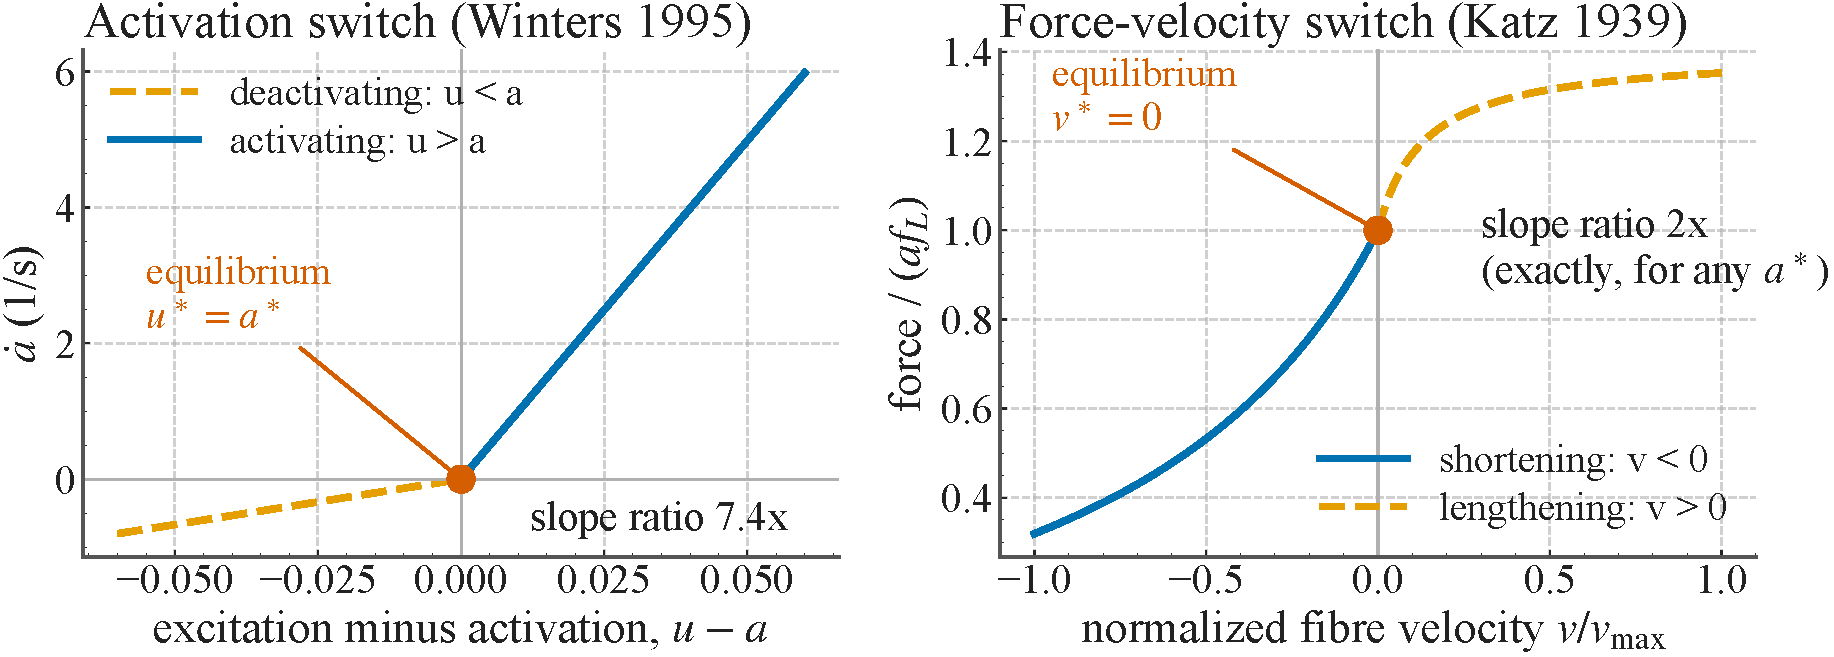
\includegraphics[width=0.58\linewidth]{fig1_kinks.pdf}
\caption{At the reference equilibrium, activation slopes differ by
7.45$\times$ and force--velocity slopes by 2$\times$.
The local model depends on the direction of the perturbation.}
\end{figure}
\end{block}

\begin{columns}[t,totalwidth=\doublecolwidth]
\begin{column}{\colwidth}
\begin{block}{Prediction: the wrong branch costs 14--75\%}
Apply a small excitation step ($+0.01$) from equilibrium and compare each
branch's linear prediction with the nonlinear trajectory.
\begin{figure}
\centering
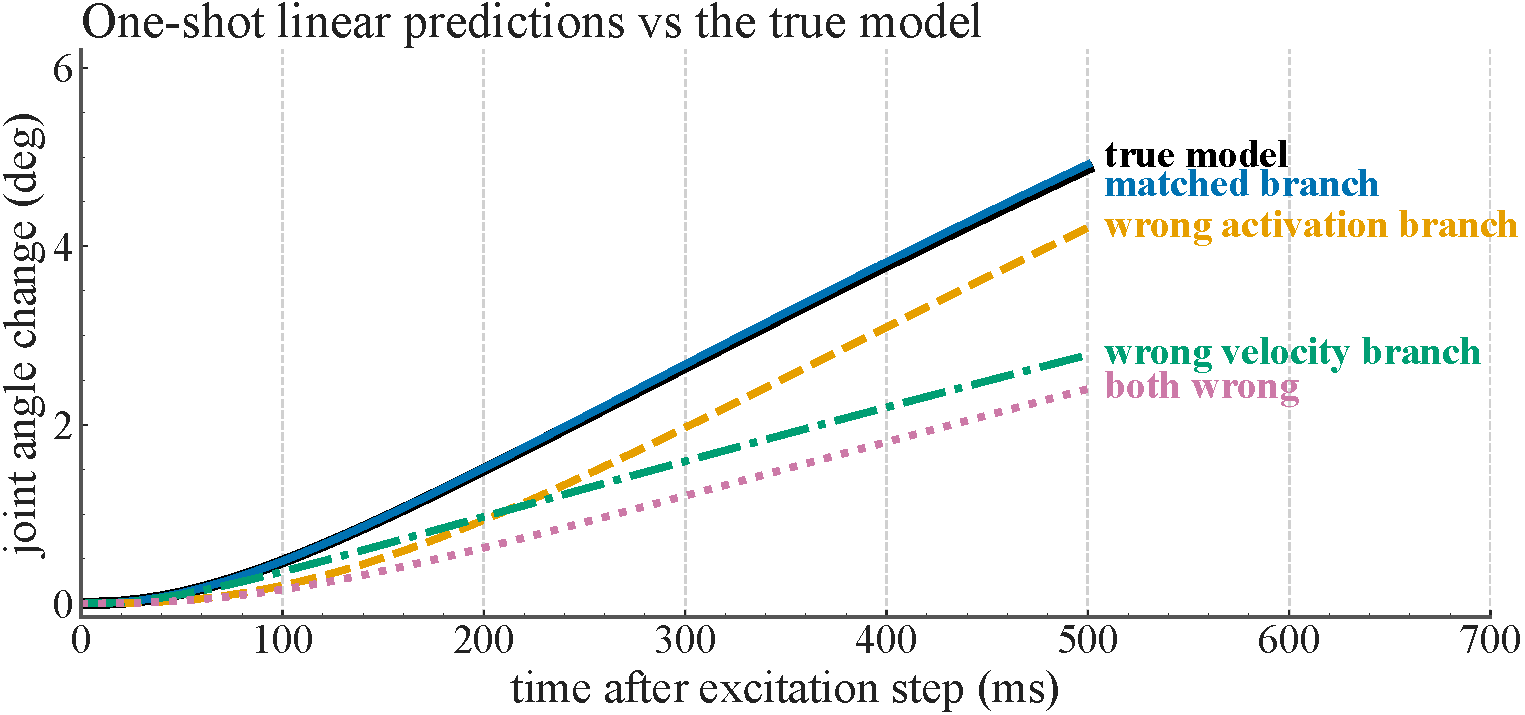
\includegraphics[width=\linewidth]{fig2_prediction.pdf}
\caption{The matched branch follows the trajectory closely;
mismatched branches diverge within 50--100\,ms.}
\end{figure}
\begin{table}
\centering
\small
\begin{tabular}{lrrrr}
\toprule
Horizon & Matched & Wrong $a$ & Wrong $v$ & Both\\
\midrule
50\,ms & 1.1\% & 71\% & 14\% & 75\%\\
100\,ms & 1.3\% & 57\% & 24\% & 67\%\\
200\,ms & 1.2\% & 38\% & 35\% & 58\%\\
500\,ms & 0.9\% & 14\% & 43\% & 51\%\\
\bottomrule
\end{tabular}
\caption{Final-angle error as a percentage of the true swing.}
\end{table}
\end{block}

\begin{block}{Across operating points}
\begin{figure}
\centering
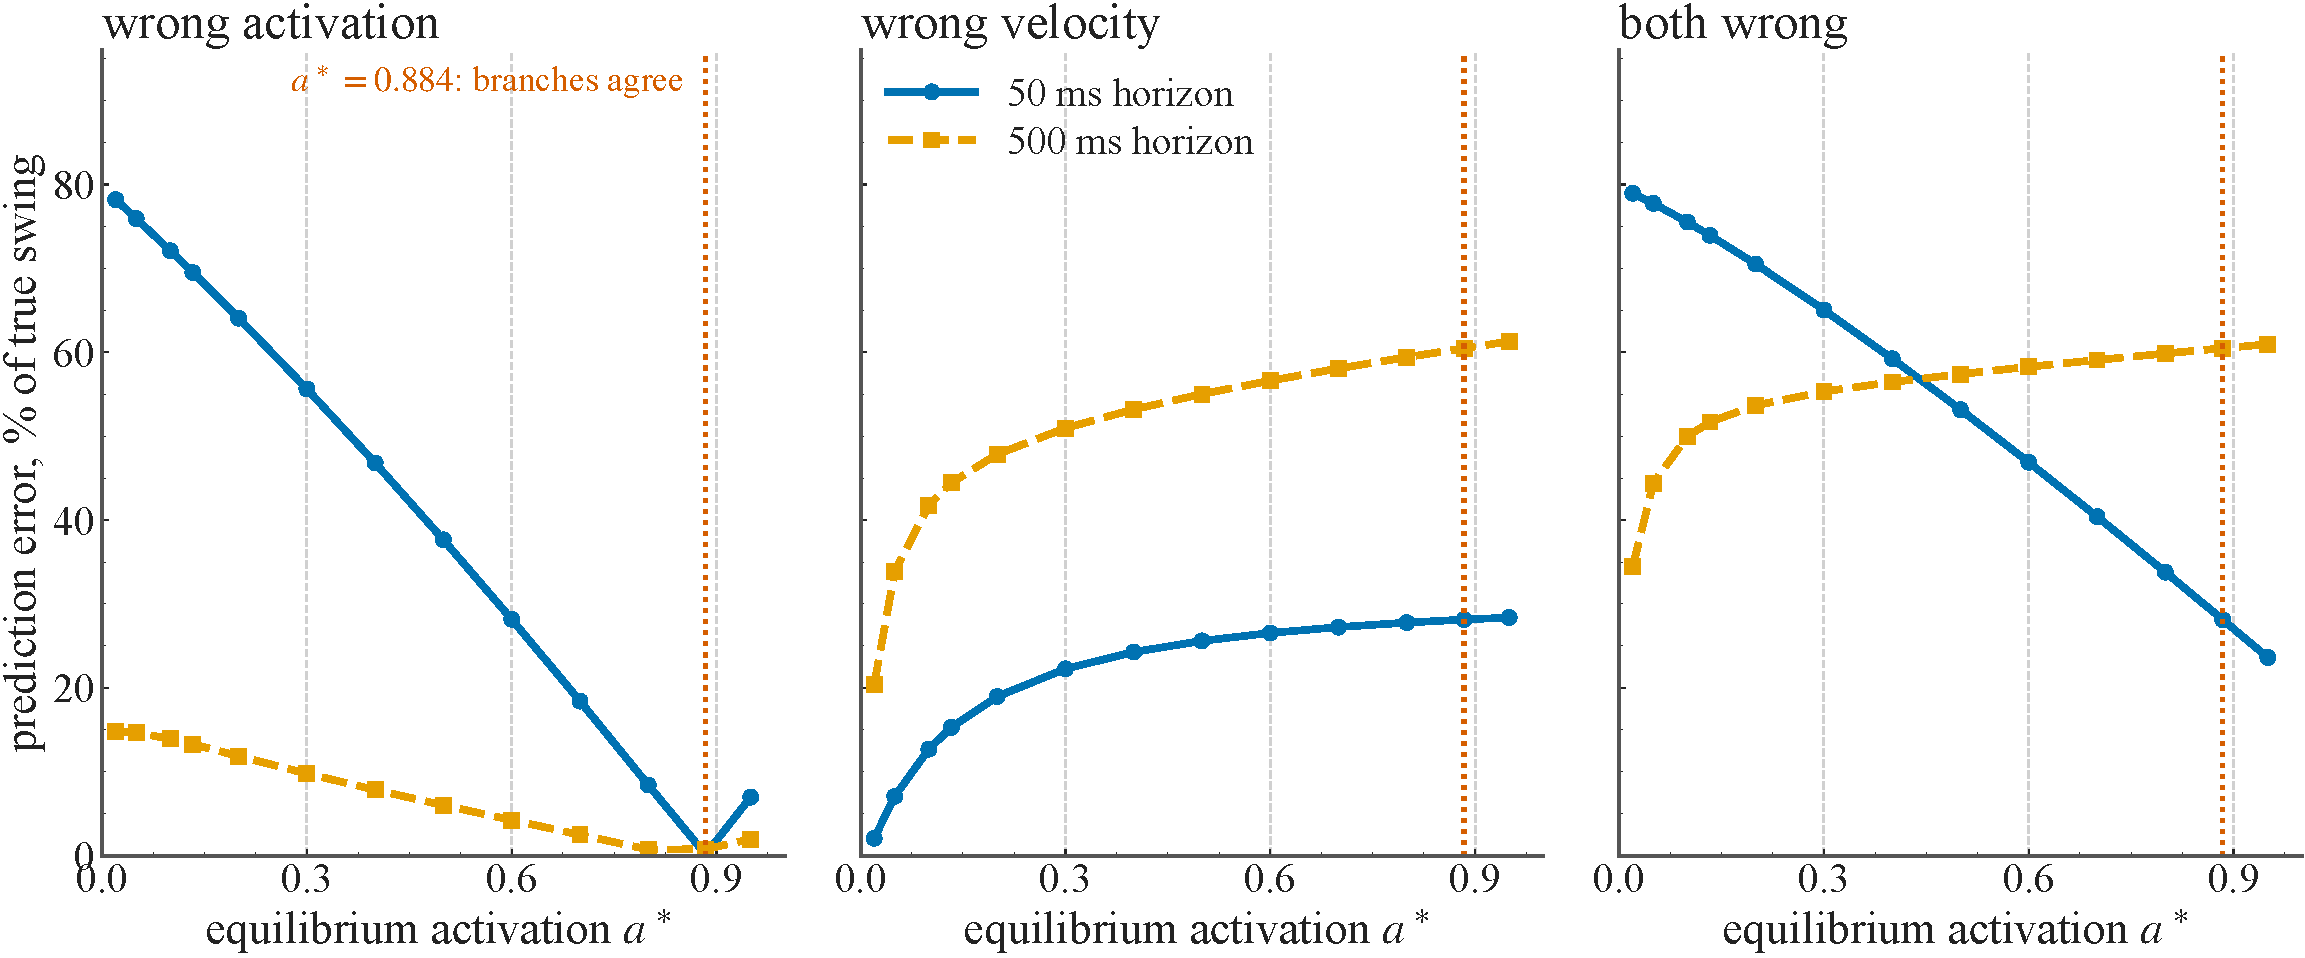
\includegraphics[width=\linewidth]{fig3_equilibria.pdf}
\caption{Held-load equilibria at 60\dg: activation-branch error falls
as activation rises, while velocity-branch error grows.}
\end{figure}
With both branches wrong, prediction error is \textbf{at least 23\%}
of the activating-step signal at every single-muscle equilibrium tested.
\end{block}

\begin{block}{Antagonist pair}
Adding triceps gives three switches and eight local modes.
\begin{figure}
\centering
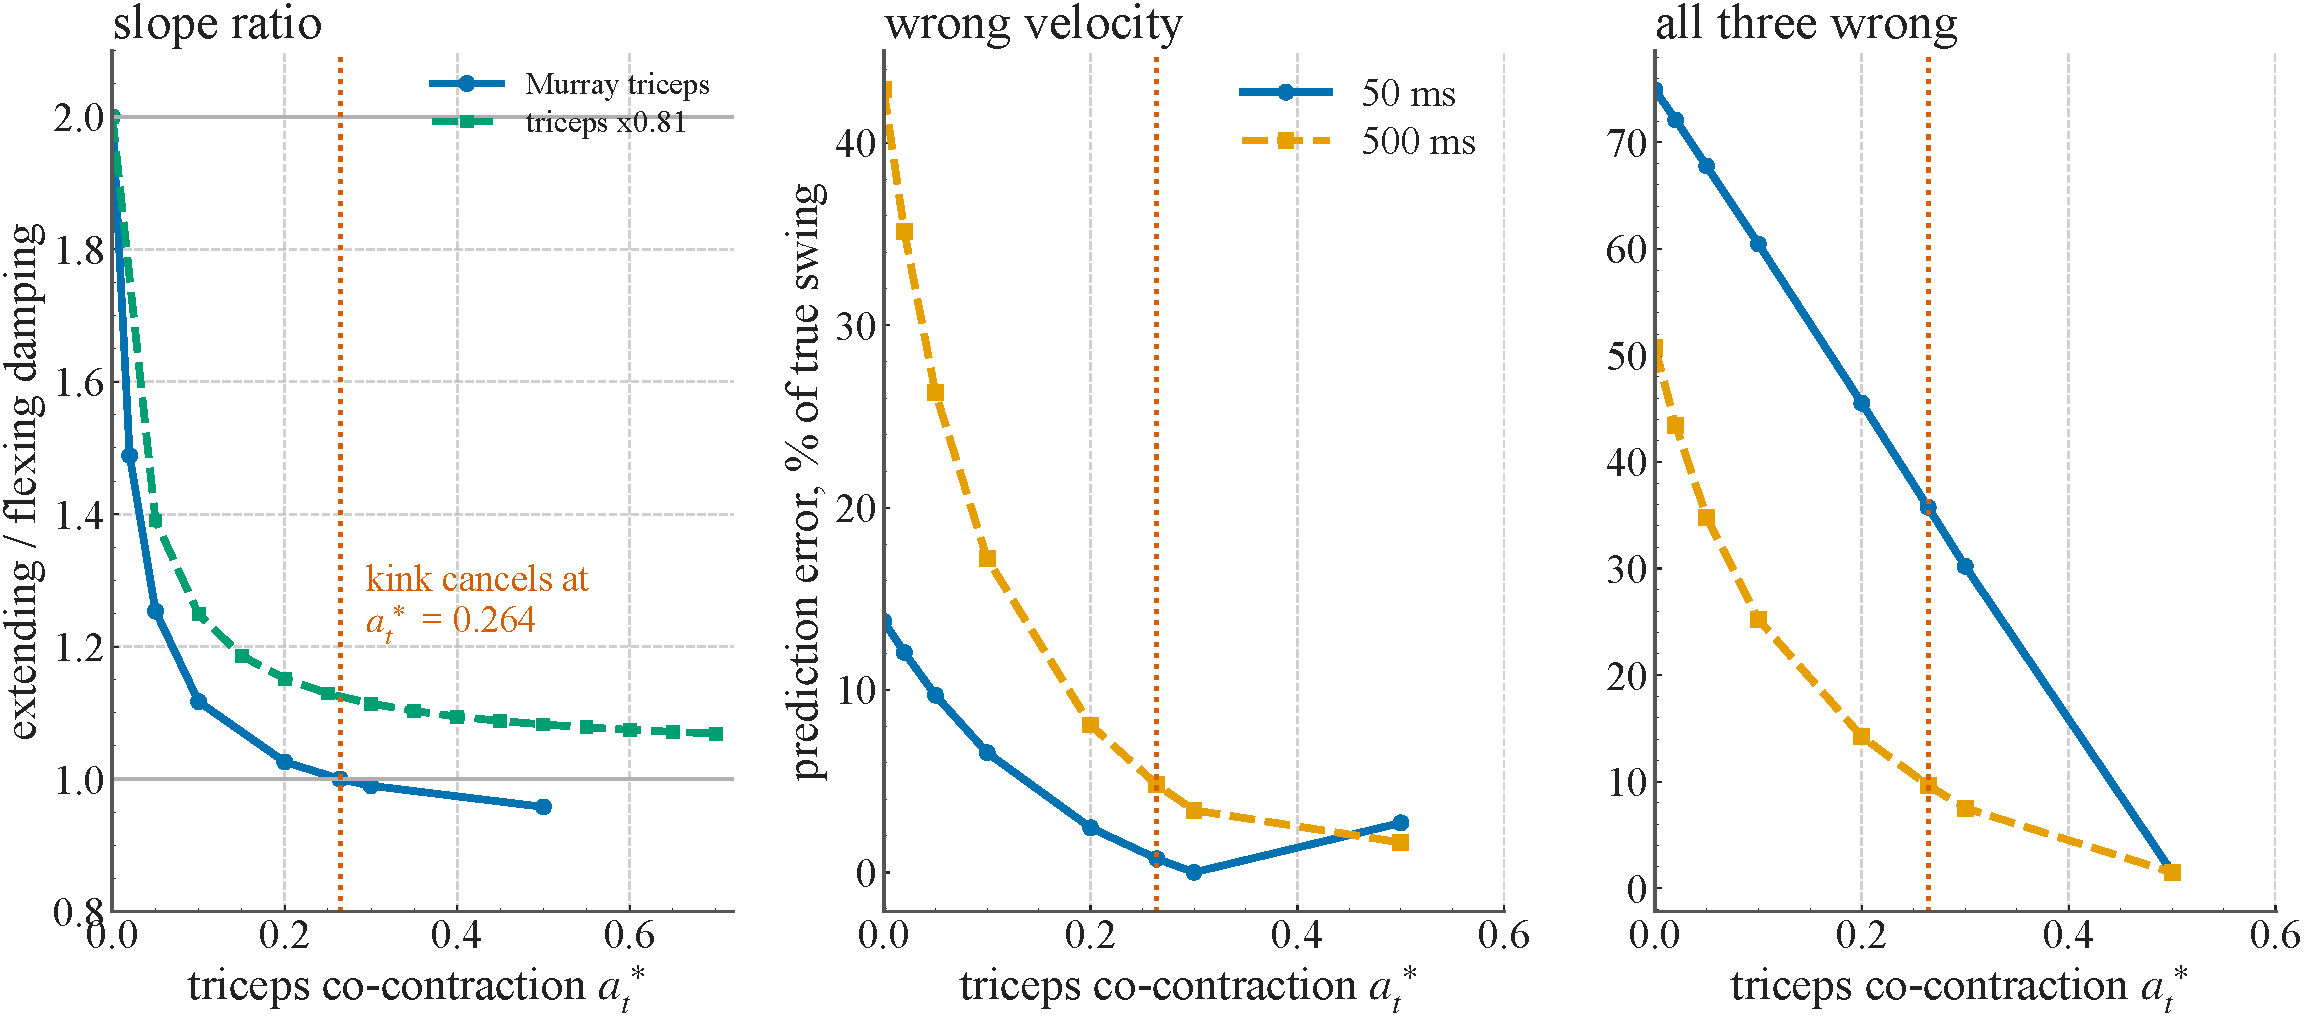
\includegraphics[width=\linewidth]{fig5_pair.pdf}
\caption{Co-contraction reduces the velocity kink, at the cost of a
second activation switch and greater effort.}
\end{figure}
The joint velocity-slope ratio approaches unity as antagonist damping
balances, with sensitivity to the triceps moment arm.
\end{block}
\end{column}
\separatorcolumn

\begin{column}{\colwidth}
\begin{block}{Feedback: transient quality matters}
Linear MPC on the nonlinear plant: $T_s=10$\,ms, horizon $N=20$, identical
weights. Only the prediction model's branch and linearization point change.
\begin{figure}
\centering
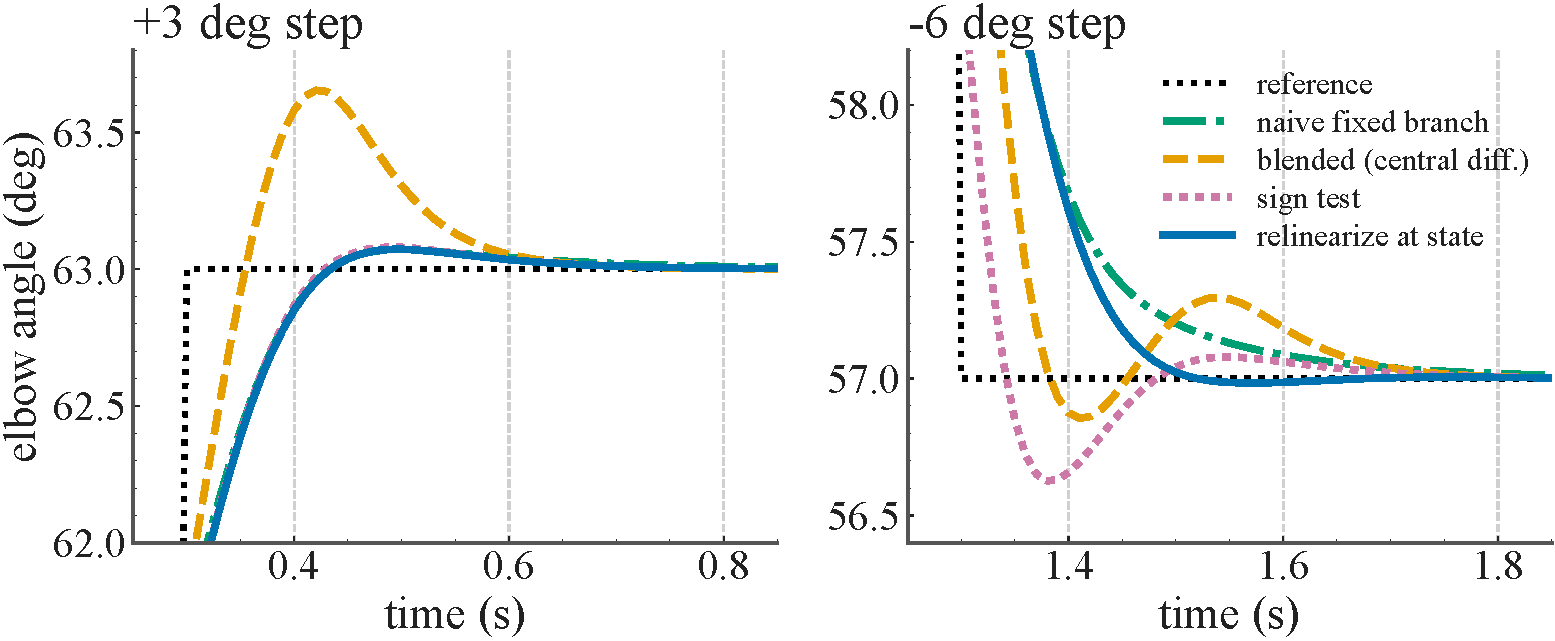
\includegraphics[width=\linewidth]{fig4_closedloop.pdf}
\caption{Tracking 60 $\to$ 63 $\to$ 57\dg.
Relinearizing reduces the lowering-step overshoot.}
\end{figure}
\end{block}

\begin{alertblock}{Closed-loop results}
\begin{table}
\centering
\small
\begin{tabular}{lrrr}
\toprule
Rule & Up overshoot & Down overshoot & Sine RMS\\
\midrule
Blended & 0.65 & 0.15 & 0.196\\
Smoothed act. & 0.42 & 0.48 & 0.169\\
Naive fixed & 0.07 & 0.00 & 0.200\\
Sign test & 0.08 & 0.37 & 0.153\\
Relinearize & 0.07 & 0.02 & 0.149\\
\bottomrule
\end{tabular}
\caption{Angles in degrees; baseline controller weights.}
\end{table}
The blended model gives \textbf{8--9$\times$ more raising overshoot}
than the bottom three rules. Smoothing only activation retains much of
the cost.

During lowering, braking re-activates the muscle mid-plan:
\textbf{0.37\dg\ overshoot with the sign test, versus 0.02\dg\ with
relinearization.}
\end{alertblock}

\begin{block}{Robustness and limitations}
\begin{itemize}
\item The overshoot pattern persists across tested sample times, noise,
activation estimates and plant mismatch.
\item Unmodelled delay can destabilize the loop; a predictor restored
stability in the tested 20 and 50\,ms cases.
\item Sinusoidal-tracking rankings depend on controller weights and noise;
relinearization is not uniformly best.
\item One simulated joint; no reflexes, short-range stiffness or history
dependence. Hardware validation remains open.
\end{itemize}
\end{block}

\begin{block}{Selected references}
{\small
Thelen (2003), \emph{J Biomech Eng} 125:70--77.\\
Katz (1939), \emph{J Physiol} 96:45--64.\\
Holzbaur et al.\ (2005), \emph{Ann Biomed Eng} 33:829--840.\\
Murray et al.\ (1995), \emph{J Biomech} 28:513--525.\\
Camlibel et al.\ (2008), \emph{Automatica} 44:1261--1267.\\
De Groote et al.\ (2016), \emph{Ann Biomed Eng} 44:2922--2936.
\par}
\end{block}
\end{column}
\end{columns}
\end{column}
\separatorcolumn
\end{columns}
\vfill
\centering
{\large 1st Workshop on Neuromuscular Robotics, IROS 2026 \quad | \quad Poster 5}
\end{frame}
\end{document}
